\documentclass[11pt]{article}
\usepackage{amsmath}
\usepackage{graphicx}
\usepackage{mdframed}
\usepackage[margin=0.7in]{geometry}
\usepackage[framed,numbered,autolinebreaks,useliterate]{mcode}

\begin{document}
\title{CS280 Computer Vision: HW3}
\author{Achal Dave, Richard Hwang}
\maketitle

\section{Canny Edge Detection}

\section{Texture Recognition}
\subsection{Training}
To compute textons, we use the code in Appendix Figure \ref{texton_train}. A
visualization of the 25 textons is shown in Figure \ref{texton_viz}. We did
not use every 5x5 patch; we subsampled for performance reasons. We will see
this turned out fine for our limited test set.

\begin{figure}[h!]
  \caption{Visualization of 25 Textons}
  \label{texton_viz}
  \centering
    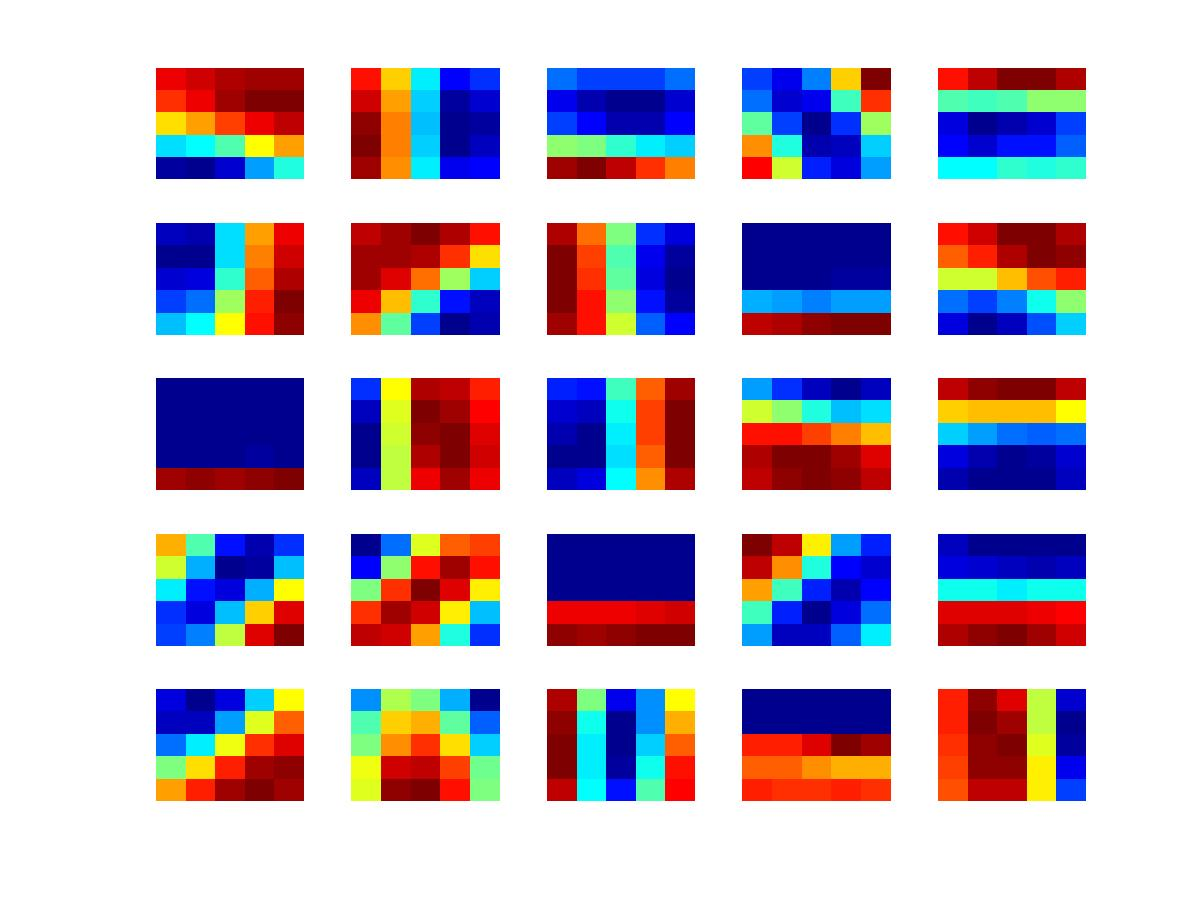
\includegraphics[width=0.6\linewidth]{../textons/textons.jpg}
\end{figure}

\subsection{Classification}
We implemented 1NN shown in Appendix Figure \ref{texton_classify}. This was
very successful. Using the script shown in Appendix Figure \ref{texton_script},
we produce the predictions shown in Figure \ref{texton_predictions}.

\begin{figure}[h!]
  \caption{Visualization of 25 Textons}
  \label{texton_viz}
  \centering
    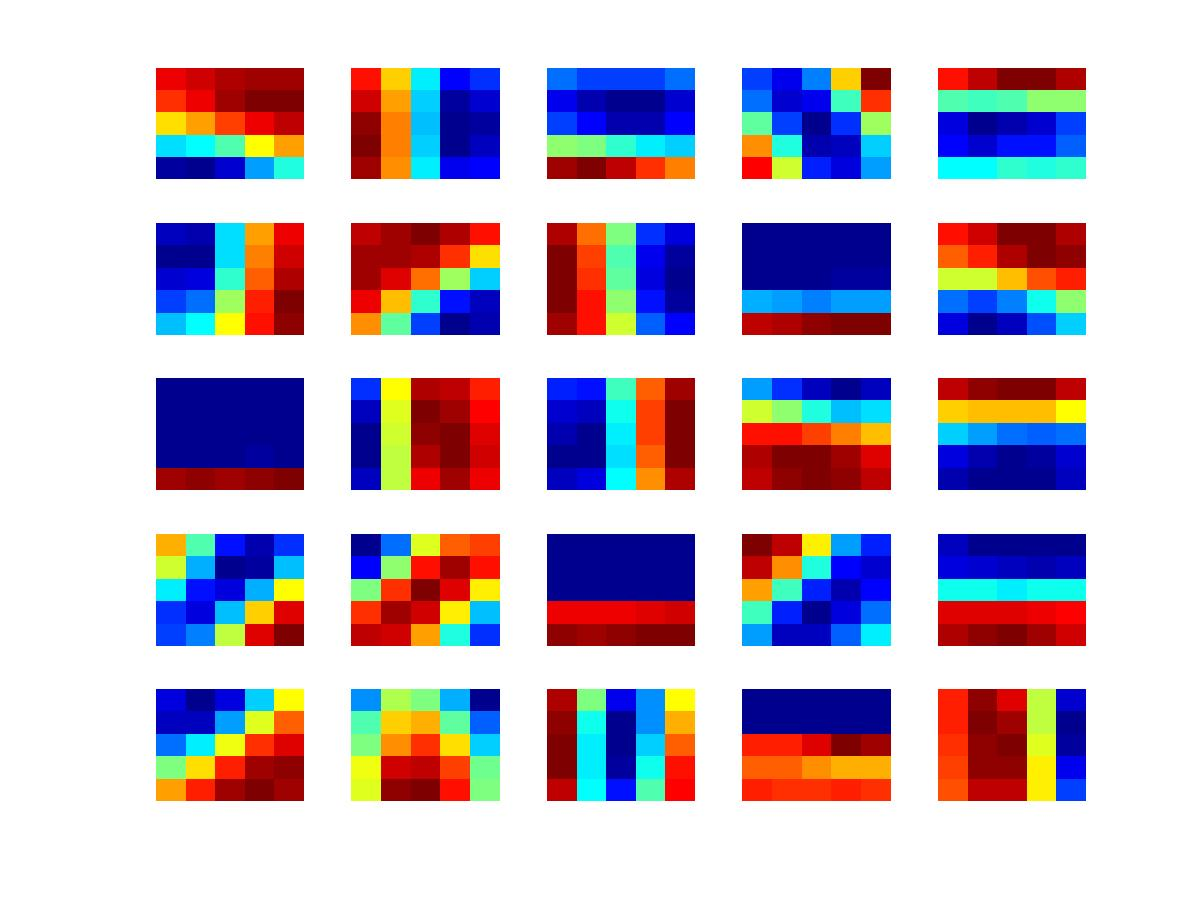
\includegraphics[width=0.6\linewidth]{../textons/textons.jpg}
\end{figure}

There was only one error: 12\_beach\_sand.tiff was predicted to have the texture
of herringbone\_weave.

\section{Block Matching}


\section{Appendix}

\begin{figure}[h!]
  \caption{Generating Images}
  \label{texton_train}
  \centering
    \begin{lstlisting}
      function [train_hists, textons, file_list] = compute_textons(k)

      patch_size = 5;
      num_patches = 30;
      texture_size = 300;
      patch_jump = texture_size / num_patches;

      patterns = dir('texture_train/*.tiff');
      file_list = {patterns.name};
      [~, n_files] = size(file_list);

      patches = zeros(n_files*num_patches*num_patches, patch_size*patch_size);
      for f_i = 1:n_files
          im = im2double(imread(sprintf('texture_train/%s', file_list{f_i})));

          for i = 1:num_patches
              for j = 1:num_patches
                  patch = im(patch_jump*(i-1)+1:patch_jump*(i-1)+5, patch_jump*(j-1)+1:patch_jump*(j-1)+5);
                  patch = (patch - mean2(patch)) / norm(patch, 1);

                  patches(num_patches*num_patches*(f_i-1)+num_patches*(i-1)+j, :) = patch(:);
              end
          end
      end

      % Cluster
      [idx, textons] = kmeans(patches, k);

      % Compute histograms for each training texture.
      train_hists = zeros(n_files,k);
      for f_i = 1:n_files
          cur_patches = patches(num_patches*num_patches*(f_i-1)+1:num_patches*num_patches*f_i, :);

          closest_textons = dsearchn(textons, cur_patches);
          histogram = histc(closest_textons, 1:k);
          histogram = histogram / norm(histogram);

          train_hists(f_i, :) = histogram';
      end
    \end{lstlisting}
\end{figure}

\begin{figure}[h!]
  \caption{Texture 1-Nearest Neighbor Classifier}
  \label{texton_classify}
  \centering
    \begin{lstlisting}
      function [f] = classify(im_name, train_hists, textons, file_list)

      im = im2double(imread(im_name));

      if nargin < 4
          [train_hists, textons, file_list] = compute_textons(25);
      end
      [n_textures, k] = size(train_hists);


      hist = create_histogram(im, textons);


      % Find nearest neighbor, using intersection kernel
      min_dist = inf;
      min_text_i = -1;

      for texture_i = 1:n_textures
          text_hist = train_hists(texture_i, :);
          dist = 0;

          for bin_i = 1:k
              dist = dist + min(hist(bin_i), text_hist(bin_i));
          end

          dist = 1 - dist;

          if dist < min_dist
              min_dist = dist;
              min_text_i = texture_i;
          end
      end

      f = figure(1);
      subplot(1,2,1);
      imshow(im);

      subplot(1,2,2);
      matched = imread(sprintf('texture_train/%s',file_list{min_text_i}));
      imshow(matched);

      disp(sprintf('%s predicted to be %s', im_name, file_list{min_text_i}));
    \end{lstlisting}
\end{figure}

\begin{figure}[h!]
  \caption{Generating all predictions}
  \label{texton_script}
  \centering
    \begin{lstlisting}
      [train_hists, textons, train_file_list] = compute_textons(25);

      test_dir = 'texture_test';

      imgs = dir(sprintf('%s/*.tiff', test_dir));
      test_file_list = {imgs.name};
      [~, n_files] = size(test_file_list);

      for test_f_i = 1:n_files
          im_name = test_file_list{test_f_i};
          test_im_name = sprintf('%s/%s', test_dir, im_name);

          fig = classify(test_im_name, train_hists, textons, train_file_list);

          result_name = sprintf('classify_results/%s.jpg', im_name);
          saveas(fig, result_name);
      end
    \end{lstlisting}
\end{figure}

\end{document}
